\documentclass[border=4pt]{standalone}
\usepackage{tikz}
\usetikzlibrary{positioning, arrows.meta, calc, fit, backgrounds}
\usepackage{amsmath}

\begin{document}
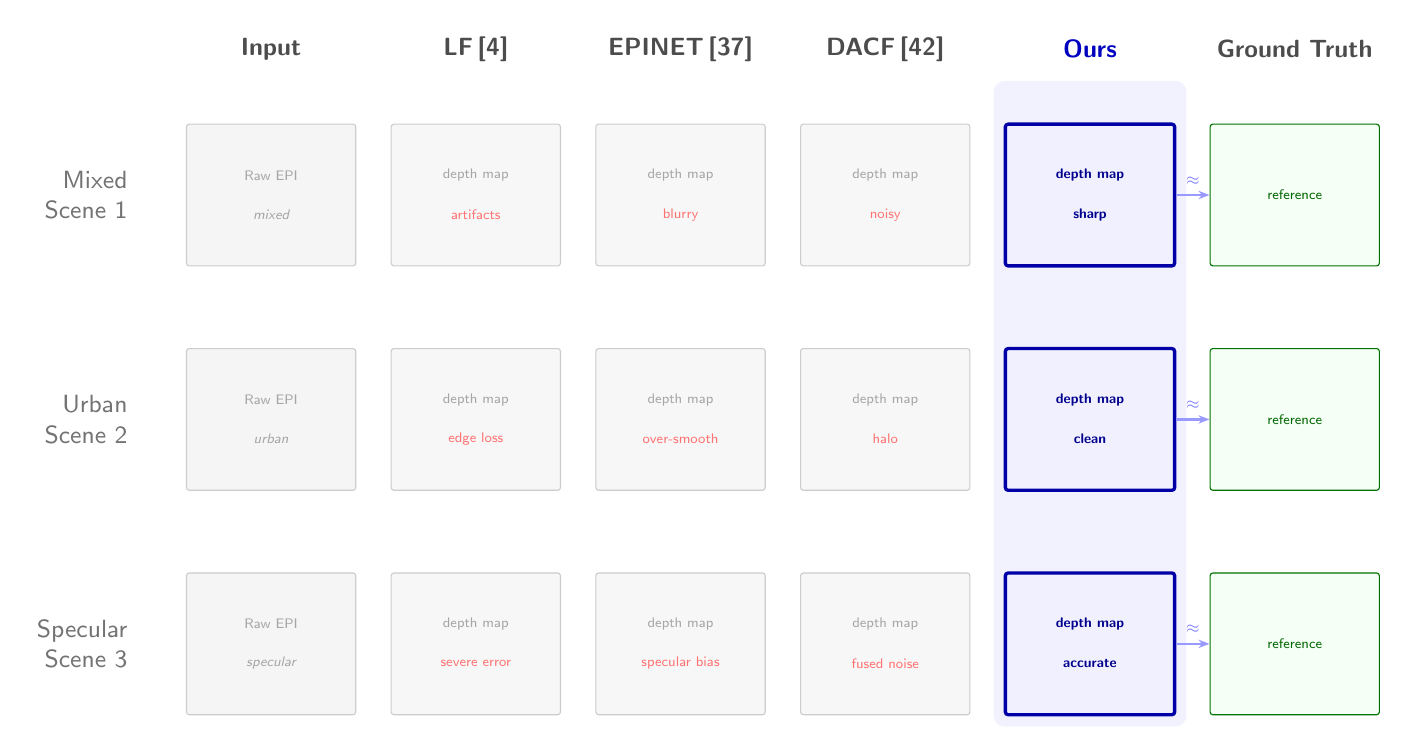
\begin{tikzpicture}[
  base/.style={
    minimum width=2.15cm, minimum height=1.8cm,
    inner sep=0pt, align=center,
    font=\sffamily\footnotesize,
    rounded corners=1pt,
  },
  inputbox/.style={base, draw=gray!40, fill=gray!8},
  methbox/.style={base, draw=gray!40, fill=gray!6},
  oursbox/.style={base, draw=blue!65!black, fill=blue!6,
    line width=1.2pt},
  gtbox/.style={base, draw=green!45!black, fill=green!4},
  collbl/.style={font=\sffamily\small\bfseries, text=black!70},
  rowlbl/.style={font=\sffamily\small, text=black!55,
    align=right, anchor=east},
  innerlbl/.style={font=\sffamily\tiny, text=black!35},
  errorlbl/.style={font=\sffamily\tiny, text=red!55},
  ours lbl/.style={font=\sffamily\tiny, text=blue!55!black},
  flowarr/.style={-{Stealth[length=4pt]}, thick, color=blue!40},
]

% Column x-positions
\def\cI{0}
\def\cA{2.6}
\def\cB{5.2}
\def\cC{7.8}
\def\cO{10.4}
\def\cG{13.0}

% Row y-positions
\def\rI{0}
\def\rII{-2.85}
\def\rIII{-5.7}

% Box dimensions
\def\bw{2.15}
\def\bh{1.8}

% ---- Background highlight for "Ours" column ----
\fill[blue!5, rounded corners=4pt]
  (\cO - \bw/2 - 0.15, \rI + \bh/2 + 0.55) rectangle
  (\cO + \bw/2 + 0.15, \rIII - \bh/2 - 0.15);

% ---- Column Headers ----
\node[collbl] at (\cI, \rI + \bh/2 + 0.95) {Input};
\node[collbl] at (\cA, \rI + \bh/2 + 0.95) {LF\,[4]};
\node[collbl] at (\cB, \rI + \bh/2 + 0.95) {EPINET\,[37]};
\node[collbl] at (\cC, \rI + \bh/2 + 0.95) {DACF\,[42]};
\node[collbl, text=blue!75!black] at (\cO, \rI + \bh/2 + 0.95) {Ours};
\node[collbl] at (\cG, \rI + \bh/2 + 0.95) {Ground Truth};

% ---- Row Labels ----
\node[rowlbl] at (-1.7, \rI) {Mixed\\Scene 1};
\node[rowlbl] at (-1.7, \rII) {Urban\\Scene 2};
\node[rowlbl] at (-1.7, \rIII) {Specular\\Scene 3};

% ======== Row 1: Mixed Scene ========
\node[inputbox] (r1I) at (\cI, \rI) {};
\node[innerlbl] at (\cI, \rI+0.25) {Raw EPI};
\node[innerlbl] at (\cI, \rI-0.25) {\itshape mixed};

\node[methbox] (r1A) at (\cA, \rI) {};
\node[innerlbl] at (\cA, \rI+0.25) {depth map};
\node[errorlbl] at (\cA, \rI-0.25) {artifacts};

\node[methbox] (r1B) at (\cB, \rI) {};
\node[innerlbl] at (\cB, \rI+0.25) {depth map};
\node[errorlbl] at (\cB, \rI-0.25) {blurry};

\node[methbox] (r1C) at (\cC, \rI) {};
\node[innerlbl] at (\cC, \rI+0.25) {depth map};
\node[errorlbl] at (\cC, \rI-0.25) {noisy};

\node[oursbox] (r1O) at (\cO, \rI) {};
\node[ours lbl] at (\cO, \rI+0.25) {\bfseries depth map};
\node[ours lbl] at (\cO, \rI-0.25) {\bfseries sharp};

\node[gtbox] (r1G) at (\cG, \rI) {};
\node[innerlbl, text=green!40!black] at (\cG, \rI) {reference};

% ======== Row 2: Urban Scene ========
\node[inputbox] (r2I) at (\cI, \rII) {};
\node[innerlbl] at (\cI, \rII+0.25) {Raw EPI};
\node[innerlbl] at (\cI, \rII-0.25) {\itshape urban};

\node[methbox] (r2A) at (\cA, \rII) {};
\node[innerlbl] at (\cA, \rII+0.25) {depth map};
\node[errorlbl] at (\cA, \rII-0.25) {edge loss};

\node[methbox] (r2B) at (\cB, \rII) {};
\node[innerlbl] at (\cB, \rII+0.25) {depth map};
\node[errorlbl] at (\cB, \rII-0.25) {over-smooth};

\node[methbox] (r2C) at (\cC, \rII) {};
\node[innerlbl] at (\cC, \rII+0.25) {depth map};
\node[errorlbl] at (\cC, \rII-0.25) {halo};

\node[oursbox] (r2O) at (\cO, \rII) {};
\node[ours lbl] at (\cO, \rII+0.25) {\bfseries depth map};
\node[ours lbl] at (\cO, \rII-0.25) {\bfseries clean};

\node[gtbox] (r2G) at (\cG, \rII) {};
\node[innerlbl, text=green!40!black] at (\cG, \rII) {reference};

% ======== Row 3: Specular Scene ========
\node[inputbox] (r3I) at (\cI, \rIII) {};
\node[innerlbl] at (\cI, \rIII+0.25) {Raw EPI};
\node[innerlbl] at (\cI, \rIII-0.25) {\itshape specular};

\node[methbox] (r3A) at (\cA, \rIII) {};
\node[innerlbl] at (\cA, \rIII+0.25) {depth map};
\node[errorlbl] at (\cA, \rIII-0.25) {severe error};

\node[methbox] (r3B) at (\cB, \rIII) {};
\node[innerlbl] at (\cB, \rIII+0.25) {depth map};
\node[errorlbl] at (\cB, \rIII-0.25) {specular bias};

\node[methbox] (r3C) at (\cC, \rIII) {};
\node[innerlbl] at (\cC, \rIII+0.25) {depth map};
\node[errorlbl] at (\cC, \rIII-0.25) {fused noise};

\node[oursbox] (r3O) at (\cO, \rIII) {};
\node[ours lbl] at (\cO, \rIII+0.25) {\bfseries depth map};
\node[ours lbl] at (\cO, \rIII-0.25) {\bfseries accurate};

\node[gtbox] (r3G) at (\cG, \rIII) {};
\node[innerlbl, text=green!40!black] at (\cG, \rIII) {reference};

% ======== Flow arrows: Ours -> GT ========
\draw[flowarr] (r1O.east) -- 
  node[above, font=\sffamily\tiny, text=blue!50] {$\approx$} (r1G.west);
\draw[flowarr] (r2O.east) -- 
  node[above, font=\sffamily\tiny, text=blue!50] {$\approx$} (r2G.west);
\draw[flowarr] (r3O.east) -- 
  node[above, font=\sffamily\tiny, text=blue!50] {$\approx$} (r3G.west);

\end{tikzpicture}
\end{document}